\documentclass[xcolor=dvipsnames,compress,t,pdf,9pt]{beamer}
\input{template_presentation}
\usepackage{polyglossia}
\setdefaultlanguage{sanskrit}
\setotherlanguage{english}

\usepackage{fontspec}
\setmainfont{Segoe UI}

% Devanagari Fonts
% \newfontfamily\devanagarifont[Scale=MatchUppercase]{Nakula}
\newfontfamily\devanagarifont[Script=Devanagari]{Nakula}
\newfontfamily\devanagarifontsf[Script=Devanagari]{Nakula}
\newfontfamily\devanagarifonttt[Script=Devanagari]{Nakula}
\newfontfamily\devtransl[Mapping=DevRom]{Segoe UI}

% Sharada Fonts
\newfontfamily\sharadafont[Script=Sharada]{Noto Sans Sharada}

\graphicspath{{images/}}
\title[\insertframenumber /\inserttotalframenumber]{Introduction to Sharada Script}


\begin{document}

	\begin{frame}
	\titlepage
	\end{frame}
	
	\section[Intro]{Introduction}
%%%%%%%%%%%%%%%%%%%%%%%%%%%%%%%%%%%%%%%%%%%%%%%%%%%%%%%%%%%%%%%%%%%%%%%%%%%%%%%%%%
\begin{frame}[fragile]\frametitle{}
\begin{center}
{\Large Introduction}
\end{center}
\end{frame}


%%%%%%%%%%%%%%%%%%%%%%%%%%%%%%%%%%%%%%%%%%%%%%%%%%%%%%%%%%%
\begin{frame}[fragile]\frametitle{Prayer}

{\sharadafont 𑆤𑆩𑆯𑇀𑆯𑆳𑆫𑆢𑆳𑆪𑆽 𑆤𑆩𑆱𑇀𑆠𑆼 𑆯𑆳𑆫𑆢𑆼 𑆢𑆼𑆮𑆴 𑆑𑆳𑆯𑇀𑆩𑆵𑆫𑆥𑆶𑆫𑆮𑆳𑆱𑆴𑆤𑆴 𑇅 𑆠𑇀𑆮𑆳𑆩𑆲𑆁 𑆥𑇀𑆫𑆳𑆫𑇀𑆡𑆪𑆼 𑆤𑆴𑆠𑇀𑆪𑆁 𑆮𑆴𑆢𑇀𑆪𑆳𑆢𑆳𑆤𑆁 𑆖 𑆢𑆼𑆲𑆴 𑆩𑆼 𑇆}

नमस्ते शारदे देवि काश्मीरपुरवासिनि । त्वामहं प्रार्थये नित्यं विद्यादानं च देहि मे ॥

namaste śārade devi kāśmīrapuravāsini . tvāmahaṃ prārthaye nityaṃ vidyādānaṃ ca dehi me ..

\end{frame}

%%%%%%%%%%%%%%%%%%%%%%%%%%%%%%%%%%%%%%%%%%%%%%%%%%%%%%%%%%%
\begin{frame}[fragile]\frametitle{Sarada Script}

\begin{itemize}
    \item Sarada script is a writing system used for the Kashmiri language by the educated Hindu minority in Kashmir and surrounding valleys.
    \item It is taught in Hindu schools but is not used in printing books.
    \item Originating in the 8th century AD, Sarada descended from the Gupta script of North India.
    \item Devanāgarī also developed from the Gupta script.
    \item The earliest inscriptions in Sarada script, found in Kashmir and northeastern Punjab, are dated AD 804.
    \item Sarada script corresponds letter for letter with Devanāgarī but differs greatly in shape with stiff, thick strokes.
    \item Muslims in Kashmir use a Persian-Arabic script.
    \item Much Kashmiri literature is written in Sanskrit using Devanāgarī script.
\end{itemize}

\end{frame}

%%%%%%%%%%%%%%%%%%%%%%%%%%%%%%%%%%%%%%%%%%%%%%%%%%%%%%%%%%%
\begin{frame}[fragile]\frametitle{Vowels}

	\begin{center}
	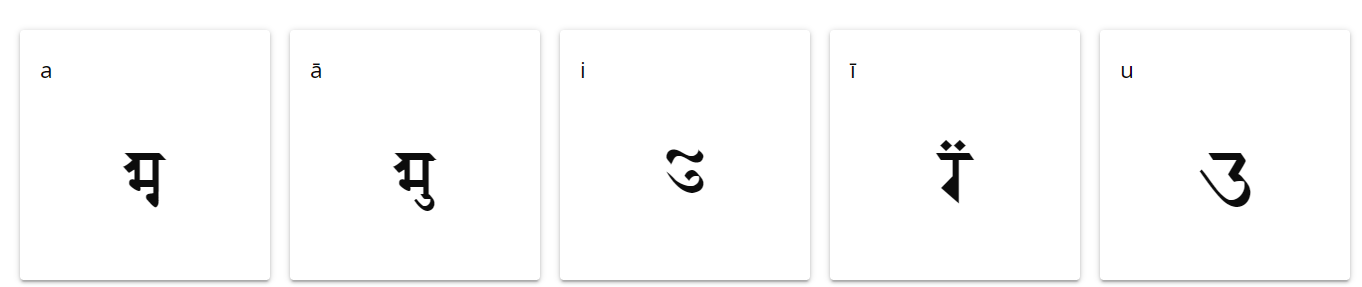
\includegraphics[width=\linewidth,keepaspectratio]{sharada_vowels_1} 
	
	{\tiny (Ref: Aksharamukha : Script Converter)}
	\end{center}	

\end{frame}

%%%%%%%%%%%%%%%%%%%%%%%%%%%%%%%%%%%%%%%%%%%%%%%%%%%%%%%%%%%
\begin{frame}[fragile]\frametitle{Vowels}

	\begin{center}
	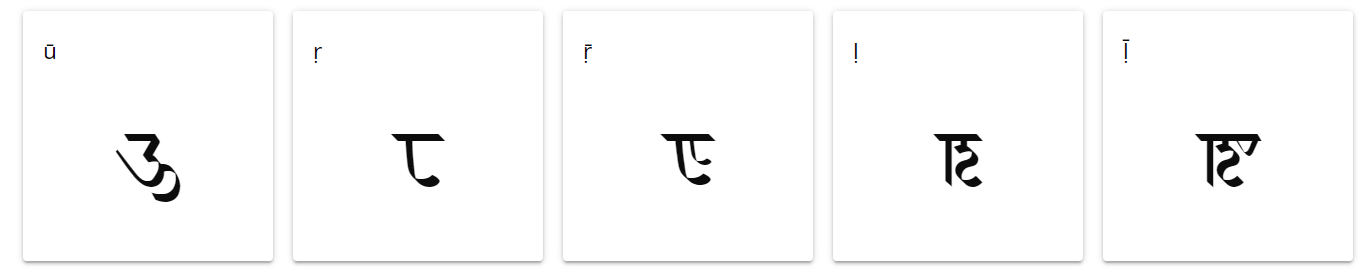
\includegraphics[width=\linewidth,keepaspectratio]{sharada_vowels_2} 
	
	{\tiny (Ref: Aksharamukha : Script Converter)}
	\end{center}	

\end{frame}

%%%%%%%%%%%%%%%%%%%%%%%%%%%%%%%%%%%%%%%%%%%%%%%%%%%%%%%%%%%
\begin{frame}[fragile]\frametitle{Vowels}

	\begin{center}
	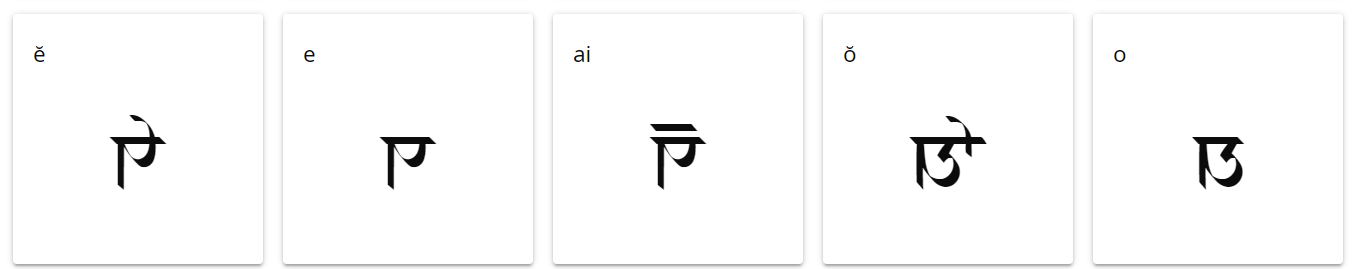
\includegraphics[width=\linewidth,keepaspectratio]{sharada_vowels_3} 
	
	{\tiny (Ref: Aksharamukha : Script Converter)}
	\end{center}	

\end{frame}

%%%%%%%%%%%%%%%%%%%%%%%%%%%%%%%%%%%%%%%%%%%%%%%%%%%%%%%%%%%
\begin{frame}[fragile]\frametitle{Vowels}

	\begin{center}
	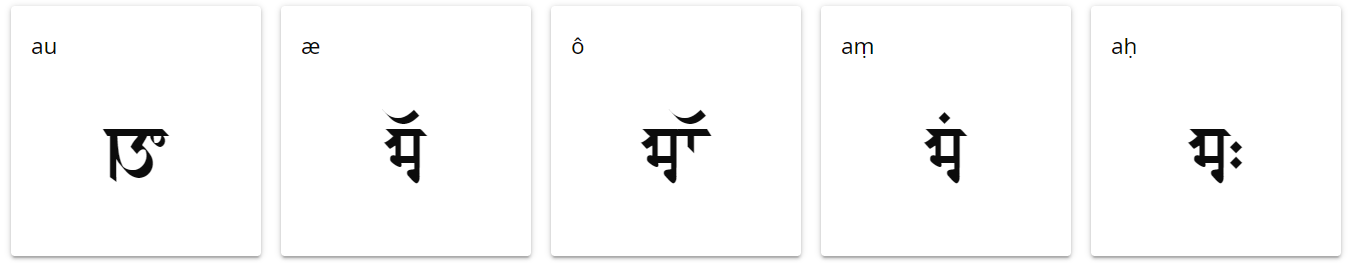
\includegraphics[width=\linewidth,keepaspectratio]{sharada_vowels_4} 
	
	{\tiny (Ref: Aksharamukha : Script Converter)}
	\end{center}	

\end{frame}

%%%%%%%%%%%%%%%%%%%%%%%%%%%%%%%%%%%%%%%%%%%%%%%%%%%%%%%%%%%
\begin{frame}[fragile]\frametitle{Vowels}

	\begin{center}
	
\includegraphics[width=\linewidth,keepaspectratio]{sharada_vowels_5} 
	
	{\tiny (Ref: Aksharamukha : Script Converter)}
	\end{center}	

\end{frame}

%%%%%%%%%%%%%%%%%%%%%%%%%%%%%%%%%%%%%%%%%%%%%%%%%%%%%%%%%%%
\begin{frame}[fragile]\frametitle{Consonants}

	\begin{center}
	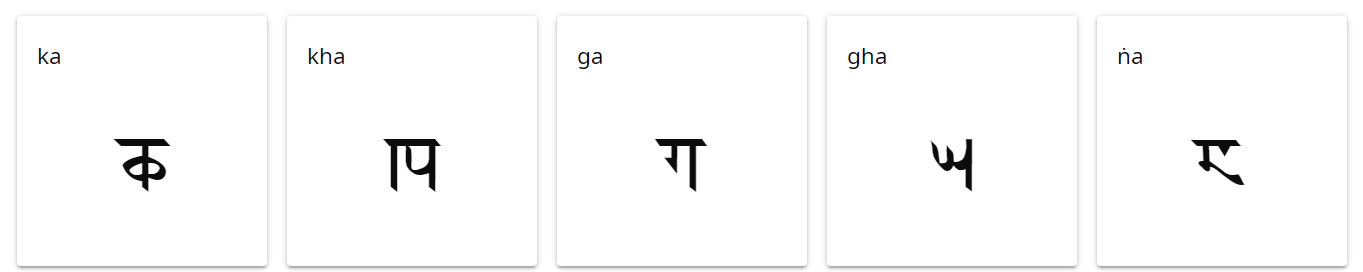
\includegraphics[width=\linewidth,keepaspectratio]{sharada_consonants_ka} 
	
	{\tiny (Ref: Aksharamukha : Script Converter)}
	\end{center}	

\end{frame}

%%%%%%%%%%%%%%%%%%%%%%%%%%%%%%%%%%%%%%%%%%%%%%%%%%%%%%%%%%%
\begin{frame}[fragile]\frametitle{Consonants}

	\begin{center}
	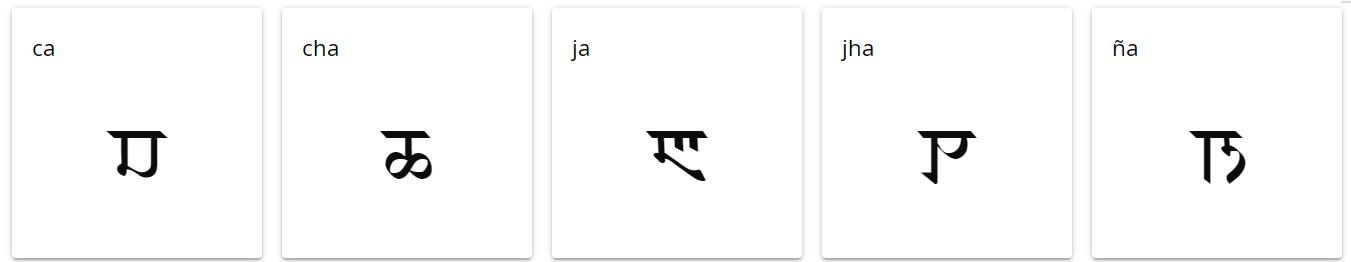
\includegraphics[width=\linewidth,keepaspectratio]{sharada_consonants_cha} 
	
	{\tiny (Ref: Aksharamukha : Script Converter)}
	\end{center}	

\end{frame}

%%%%%%%%%%%%%%%%%%%%%%%%%%%%%%%%%%%%%%%%%%%%%%%%%%%%%%%%%%%
\begin{frame}[fragile]\frametitle{Consonants}

	\begin{center}
	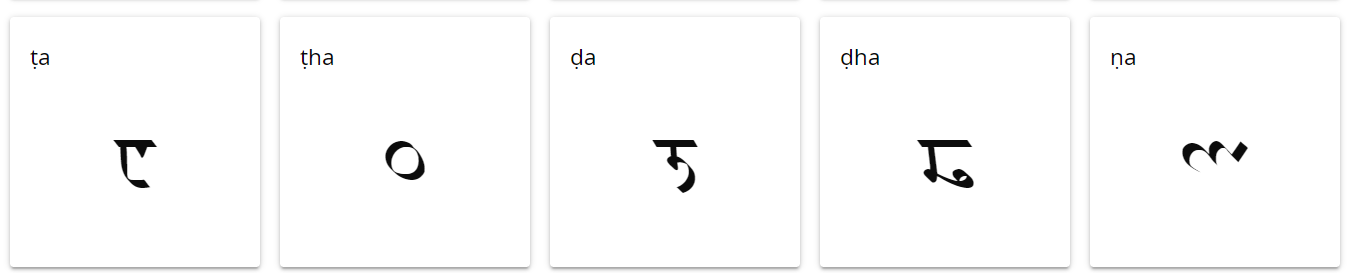
\includegraphics[width=\linewidth,keepaspectratio]{sharada_consonants_Ta} 
	
	{\tiny (Ref: Aksharamukha : Script Converter)}
	\end{center}	

\end{frame}

%%%%%%%%%%%%%%%%%%%%%%%%%%%%%%%%%%%%%%%%%%%%%%%%%%%%%%%%%%%
\begin{frame}[fragile]\frametitle{Consonants}

	\begin{center}
	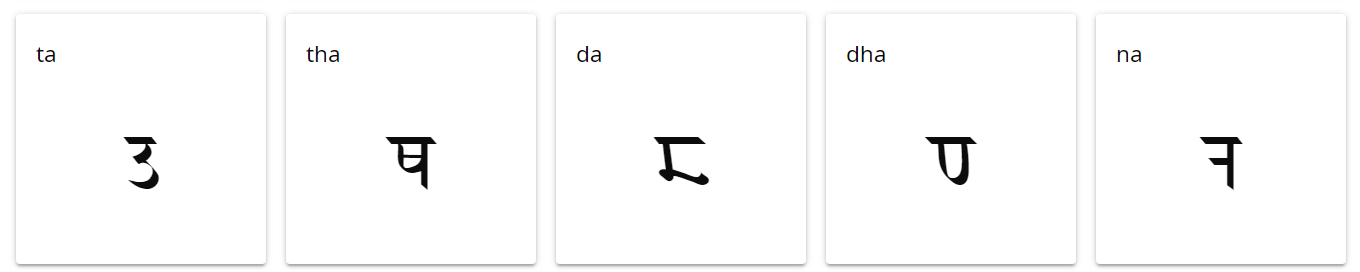
\includegraphics[width=\linewidth,keepaspectratio]{sharada_consonants_taa} 
	
	{\tiny (Ref: Aksharamukha : Script Converter)}
	\end{center}	

\end{frame}

%%%%%%%%%%%%%%%%%%%%%%%%%%%%%%%%%%%%%%%%%%%%%%%%%%%%%%%%%%%
\begin{frame}[fragile]\frametitle{Consonants}

	\begin{center}
	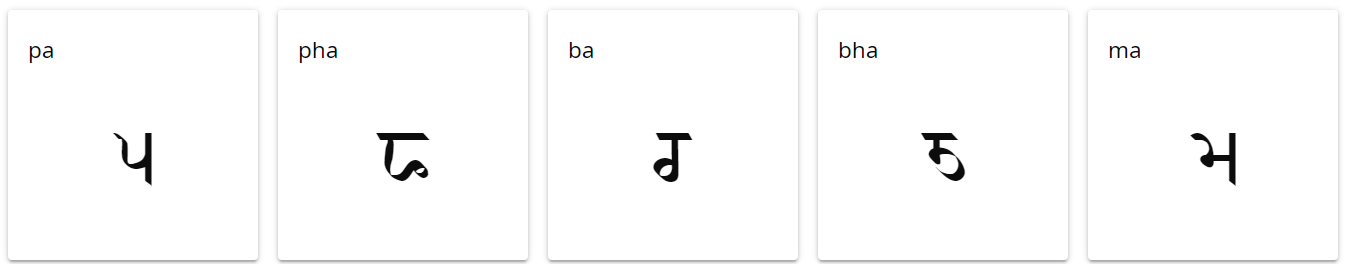
\includegraphics[width=\linewidth,keepaspectratio]{sharada_consonants_pa} 
	
	{\tiny (Ref: Aksharamukha : Script Converter)}
	\end{center}	

\end{frame}

%%%%%%%%%%%%%%%%%%%%%%%%%%%%%%%%%%%%%%%%%%%%%%%%%%%%%%%%%%%
\begin{frame}[fragile]\frametitle{Consonants}

	\begin{center}
	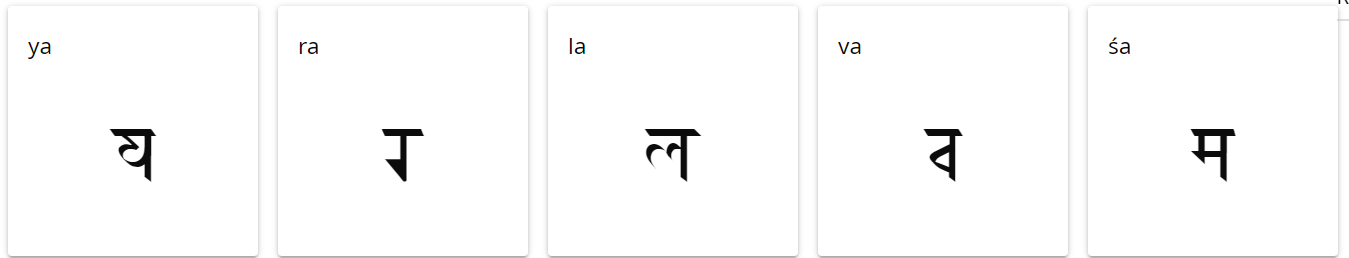
\includegraphics[width=\linewidth,keepaspectratio]{sharada_consonants_ya} 
	
	{\tiny (Ref: Aksharamukha : Script Converter)}
	\end{center}	

\end{frame}

%%%%%%%%%%%%%%%%%%%%%%%%%%%%%%%%%%%%%%%%%%%%%%%%%%%%%%%%%%%
\begin{frame}[fragile]\frametitle{Consonants}

	\begin{center}
	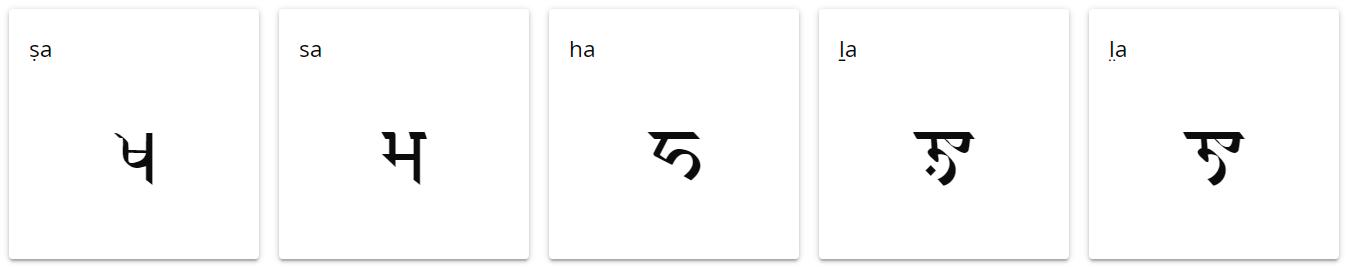
\includegraphics[width=\linewidth,keepaspectratio]{sharada_consonants_sha} 
	
	{\tiny (Ref: Aksharamukha : Script Converter)}
	\end{center}	

\end{frame}

%%%%%%%%%%%%%%%%%%%%%%%%%%%%%%%%%%%%%%%%%%%%%%%%%%%%%%%%%%%
\begin{frame}[fragile]\frametitle{Consonants}

	\begin{center}
	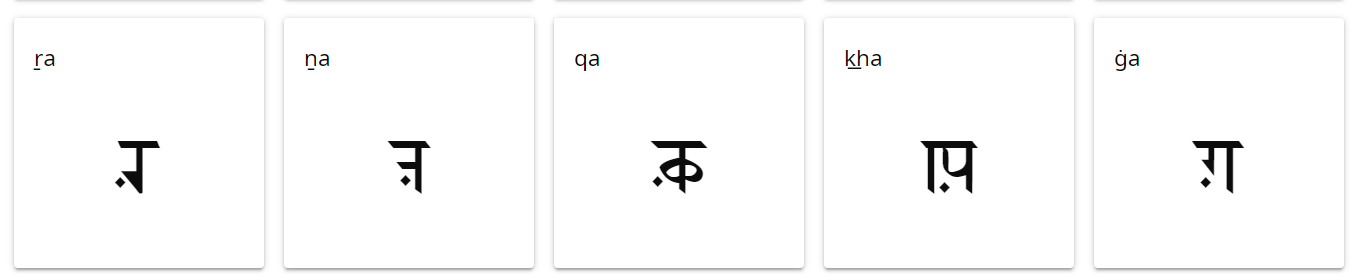
\includegraphics[width=\linewidth,keepaspectratio]{sharada_consonants_ra} 
	
	{\tiny (Ref: Aksharamukha : Script Converter)}
	\end{center}	

\end{frame}

%%%%%%%%%%%%%%%%%%%%%%%%%%%%%%%%%%%%%%%%%%%%%%%%%%%%%%%%%%%
\begin{frame}[fragile]\frametitle{Consonants}

	\begin{center}
	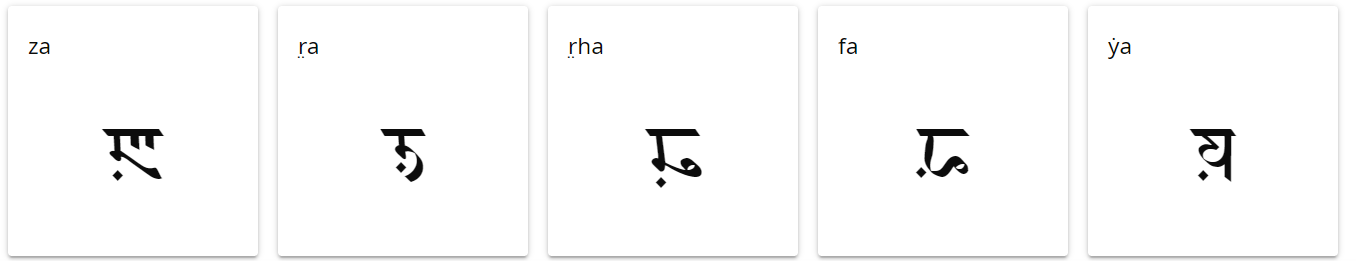
\includegraphics[width=\linewidth,keepaspectratio]{sharada_consonants_za} 
	
	{\tiny (Ref: Aksharamukha : Script Converter)}
	\end{center}	

\end{frame}

%%%%%%%%%%%%%%%%%%%%%%%%%%%%%%%%%%%%%%%%%%%%%%%%%%%%%%%%%%%
\begin{frame}[fragile]\frametitle{Compounds}

	\begin{center}
	
\includegraphics[width=\linewidth,keepaspectratio]{sharada_compounds_kaa} 
	
	{\tiny (Ref: Aksharamukha : Script Converter)}
	\end{center}	

\end{frame}

%%%%%%%%%%%%%%%%%%%%%%%%%%%%%%%%%%%%%%%%%%%%%%%%%%%%%%%%%%%
\begin{frame}[fragile]\frametitle{Compounds}

	\begin{center}
	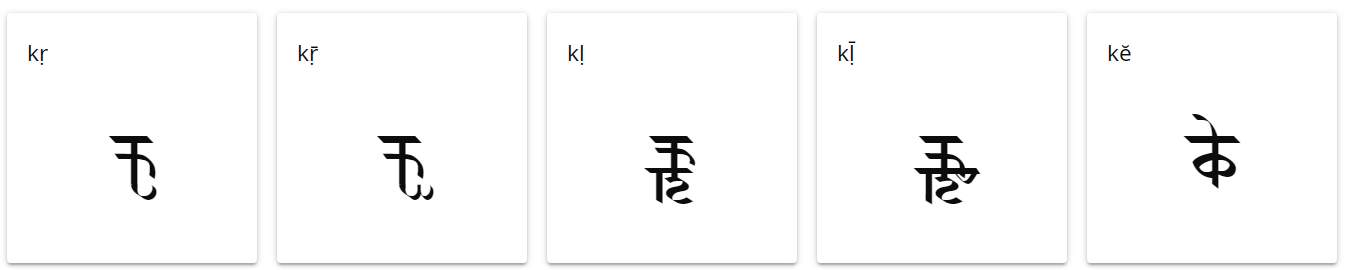
\includegraphics[width=\linewidth,keepaspectratio]{sharada_compounds_kr} 
	
	{\tiny (Ref: Aksharamukha : Script Converter)}
	\end{center}	

\end{frame}

%%%%%%%%%%%%%%%%%%%%%%%%%%%%%%%%%%%%%%%%%%%%%%%%%%%%%%%%%%%
\begin{frame}[fragile]\frametitle{Compounds}

	\begin{center}
	
\includegraphics[width=\linewidth,keepaspectratio]{sharada_compounds_ke} 
	
	{\tiny (Ref: Aksharamukha : Script Converter)}
	\end{center}	

\end{frame}

%%%%%%%%%%%%%%%%%%%%%%%%%%%%%%%%%%%%%%%%%%%%%%%%%%%%%%%%%%%
\begin{frame}[fragile]\frametitle{Compounds}

	\begin{center}
	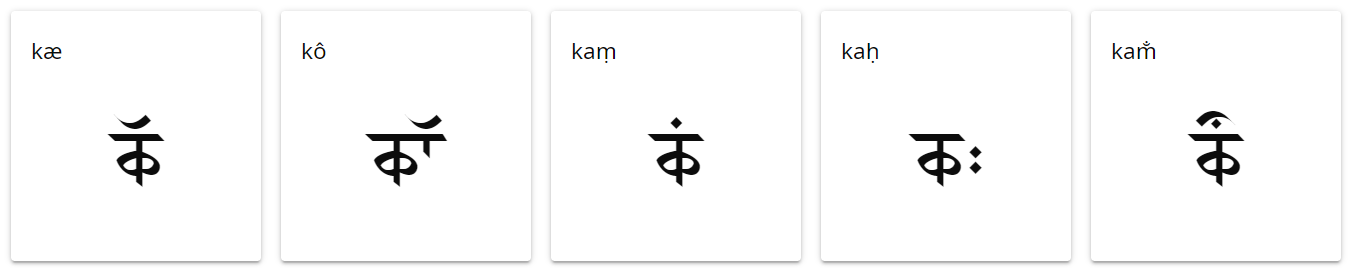
\includegraphics[width=\linewidth,keepaspectratio]{sharada_compounds_kae} 
	
	{\tiny (Ref: Aksharamukha : Script Converter)}
	\end{center}	

\end{frame}

%%%%%%%%%%%%%%%%%%%%%%%%%%%%%%%%%%%%%%%%%%%%%%%%%%%%%%%%%%%
\begin{frame}[fragile]\frametitle{Compounds}

	\begin{center}
	
\includegraphics[width=\linewidth,keepaspectratio]{sharada_compounds_k} 
	
	{\tiny (Ref: Aksharamukha : Script Converter)}
	\end{center}	

\end{frame}

%%%%%%%%%%%%%%%%%%%%%%%%%%%%%%%%%%%%%%%%%%%%%%%%%%%%%%%%%%%
\begin{frame}[fragile]\frametitle{Compounds}

	\begin{center}
	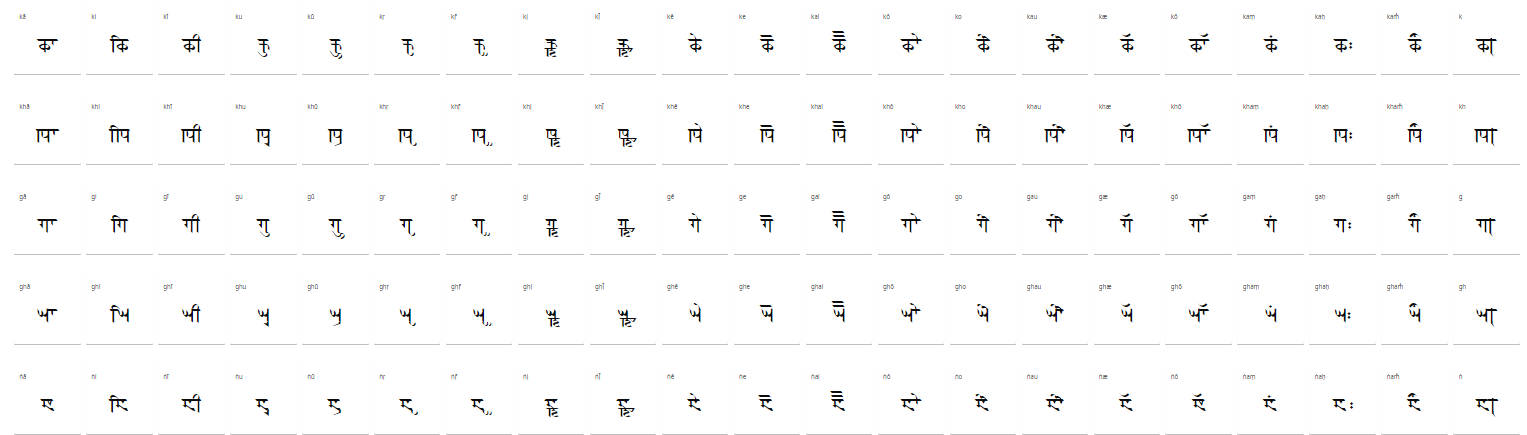
\includegraphics[width=\linewidth,keepaspectratio]{sharada_compounds_ka_varga} 
	
	{\tiny (Ref: Aksharamukha : Script Converter)}
	\end{center}	

\end{frame}

%%%%%%%%%%%%%%%%%%%%%%%%%%%%%%%%%%%%%%%%%%%%%%%%%%%%%%%%%%%
\begin{frame}[fragile]\frametitle{Compounds}

	\begin{center}
	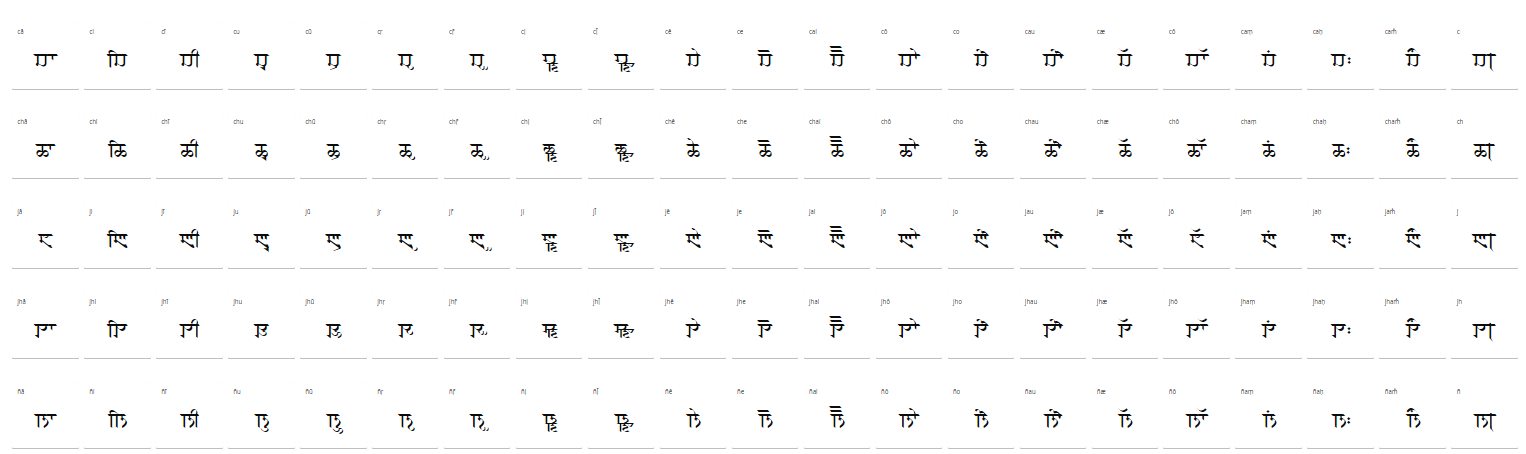
\includegraphics[width=\linewidth,keepaspectratio]{sharada_compounds_cha_varga} 
	
	{\tiny (Ref: Aksharamukha : Script Converter)}
	\end{center}	

\end{frame}

%%%%%%%%%%%%%%%%%%%%%%%%%%%%%%%%%%%%%%%%%%%%%%%%%%%%%%%%%%%
\begin{frame}[fragile]\frametitle{Compounds}

	\begin{center}
	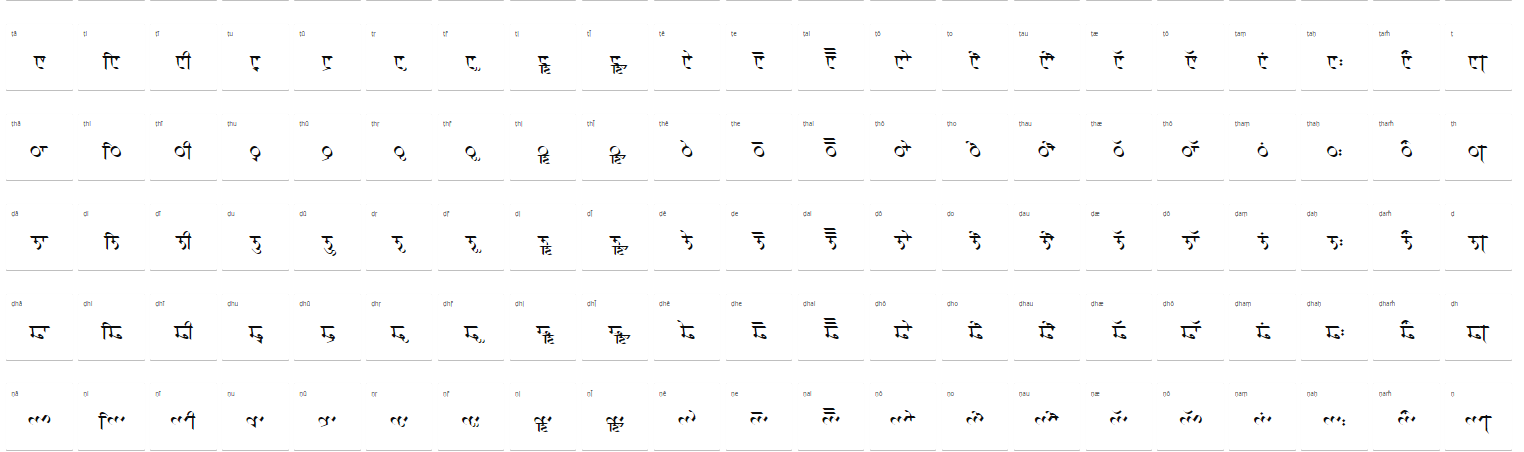
\includegraphics[width=\linewidth,keepaspectratio]{sharada_compounds_Ta_varga} 
	
	{\tiny (Ref: Aksharamukha : Script Converter)}
	\end{center}	

\end{frame}

%%%%%%%%%%%%%%%%%%%%%%%%%%%%%%%%%%%%%%%%%%%%%%%%%%%%%%%%%%%
\begin{frame}[fragile]\frametitle{Compounds}

	\begin{center}
	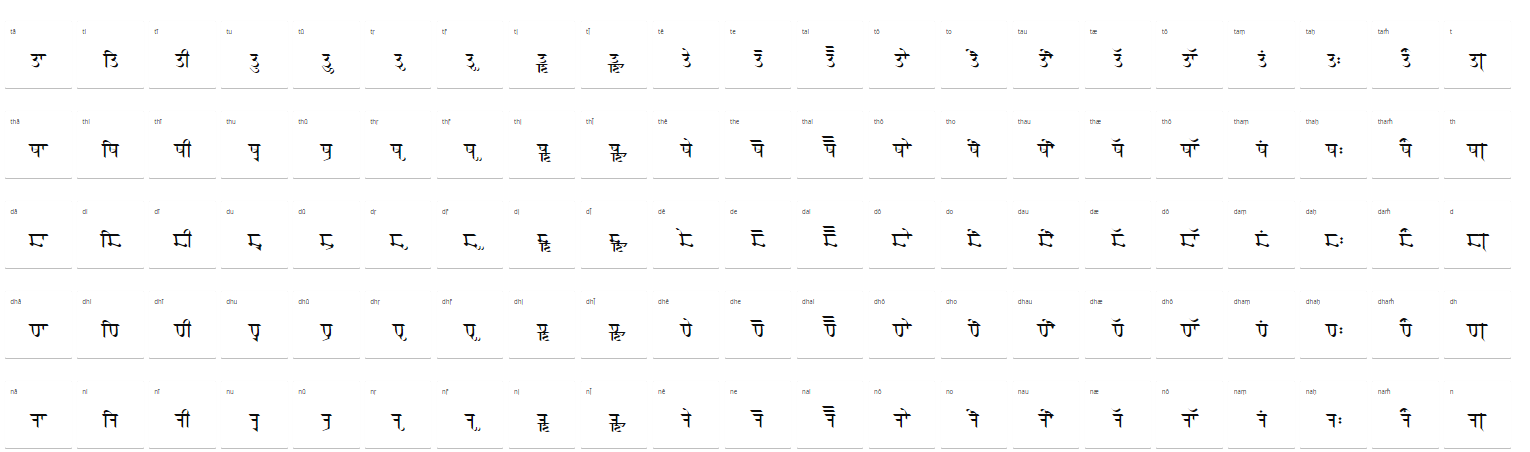
\includegraphics[width=\linewidth,keepaspectratio]{sharada_compounds_taa_varga} 
	
	{\tiny (Ref: Aksharamukha : Script Converter)}
	\end{center}	

\end{frame}

%%%%%%%%%%%%%%%%%%%%%%%%%%%%%%%%%%%%%%%%%%%%%%%%%%%%%%%%%%%
\begin{frame}[fragile]\frametitle{Compounds}

	\begin{center}
	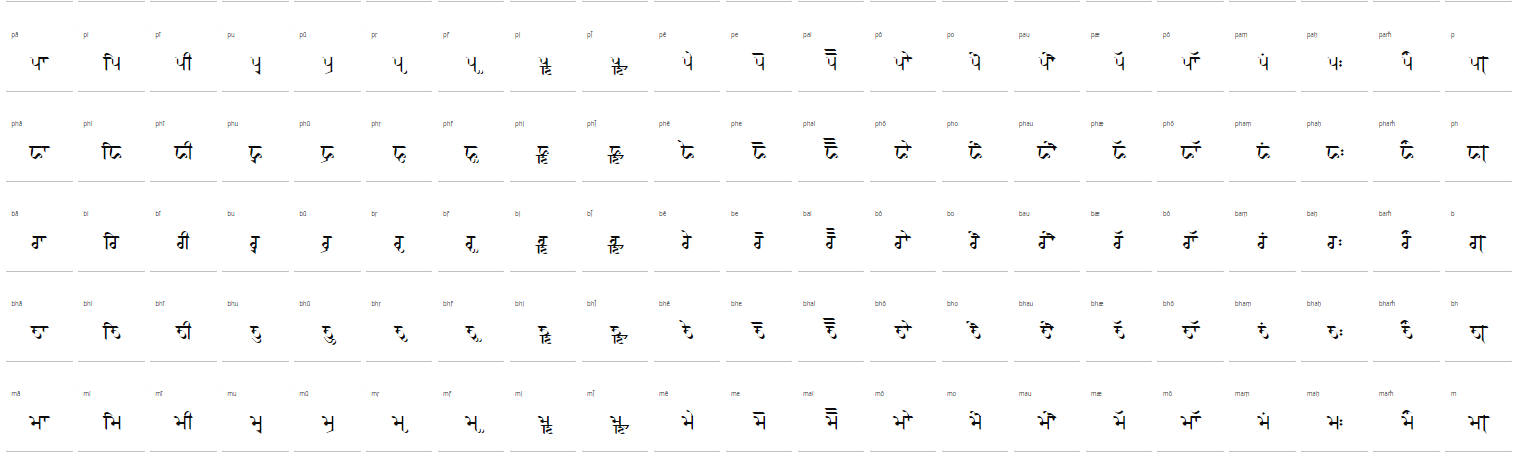
\includegraphics[width=\linewidth,keepaspectratio]{sharada_compounds_pa_varga} 
	
	{\tiny (Ref: Aksharamukha : Script Converter)}
	\end{center}	

\end{frame}

%%%%%%%%%%%%%%%%%%%%%%%%%%%%%%%%%%%%%%%%%%%%%%%%%%%%%%%%%%%
\begin{frame}[fragile]\frametitle{Compounds}

	\begin{center}
	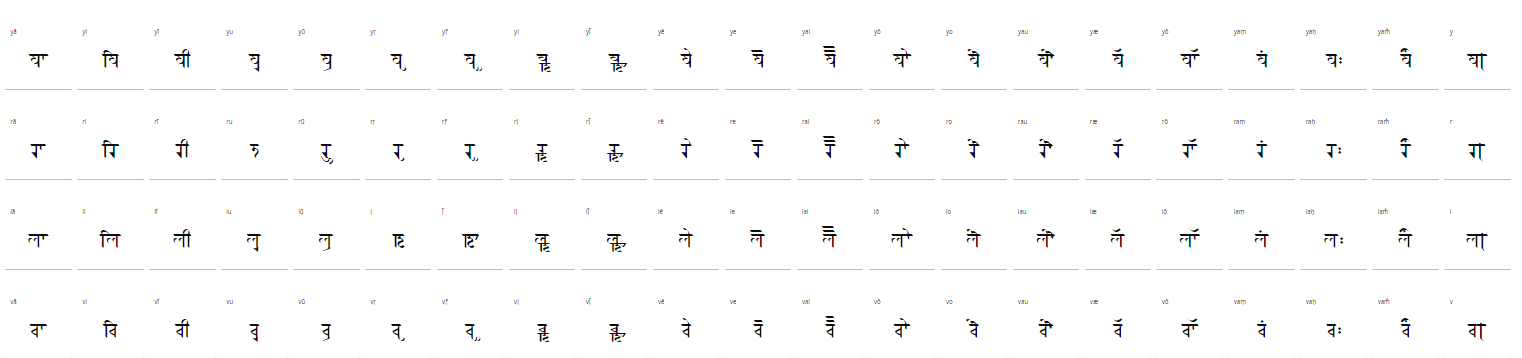
\includegraphics[width=\linewidth,keepaspectratio]{sharada_compounds_ya_varga} 
	
	{\tiny (Ref: Aksharamukha : Script Converter)}
	\end{center}	

\end{frame}

%%%%%%%%%%%%%%%%%%%%%%%%%%%%%%%%%%%%%%%%%%%%%%%%%%%%%%%%%%%
\begin{frame}[fragile]\frametitle{Compounds}

	\begin{center}
	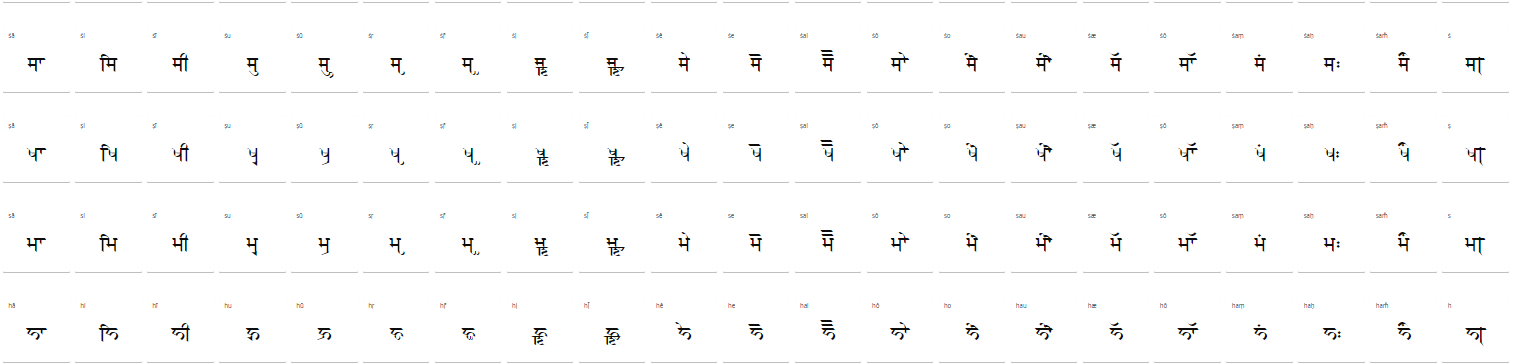
\includegraphics[width=\linewidth,keepaspectratio]{sharada_compounds_sa_varga} 
	
	{\tiny (Ref: Aksharamukha : Script Converter)}
	\end{center}	

\end{frame}

%%%%%%%%%%%%%%%%%%%%%%%%%%%%%%%%%%%%%%%%%%%%%%%%%%%%%%%%%%%
\begin{frame}[fragile]\frametitle{Compounds}

	\begin{center}
	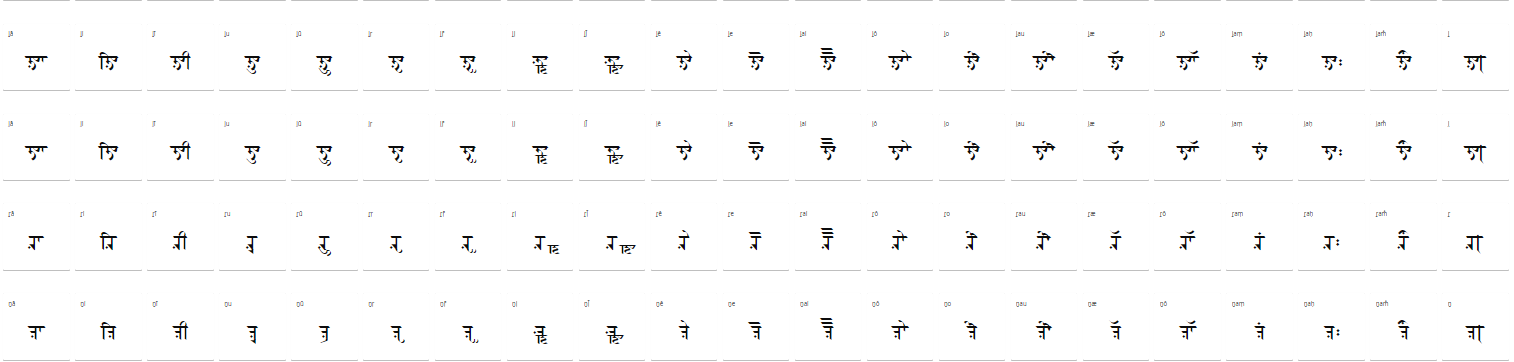
\includegraphics[width=\linewidth,keepaspectratio]{sharada_compounds_la_varga} 
	
	{\tiny (Ref: Aksharamukha : Script Converter)}
	\end{center}	

\end{frame}

%%%%%%%%%%%%%%%%%%%%%%%%%%%%%%%%%%%%%%%%%%%%%%%%%%%%%%%%%%%
\begin{frame}[fragile]\frametitle{Compounds}

	\begin{center}
	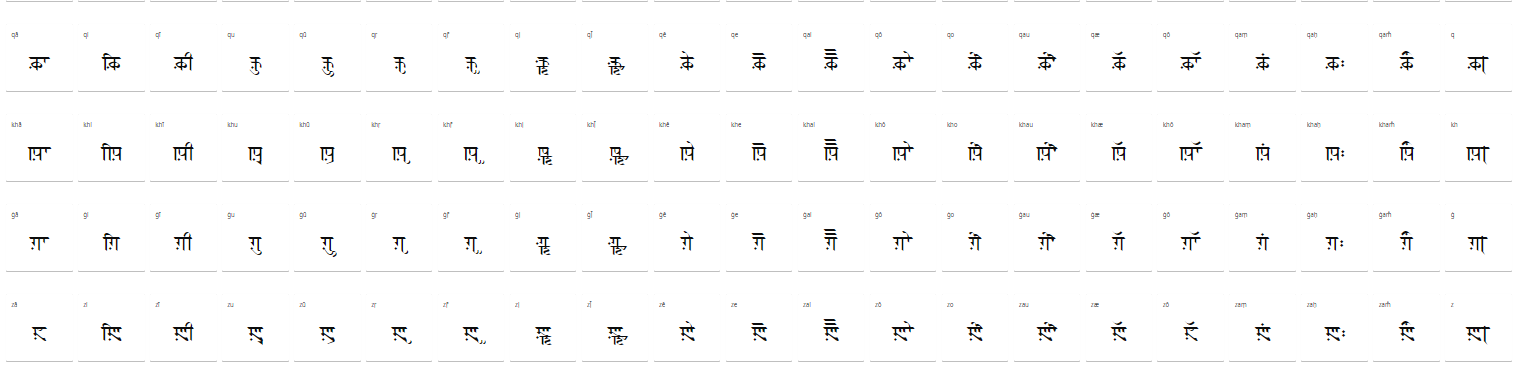
\includegraphics[width=\linewidth,keepaspectratio]{sharada_compounds_qa_varga} 
	
	{\tiny (Ref: Aksharamukha : Script Converter)}
	\end{center}	

\end{frame}

%%%%%%%%%%%%%%%%%%%%%%%%%%%%%%%%%%%%%%%%%%%%%%%%%%%%%%%%%%%
\begin{frame}[fragile]\frametitle{Compounds}

	\begin{center}
	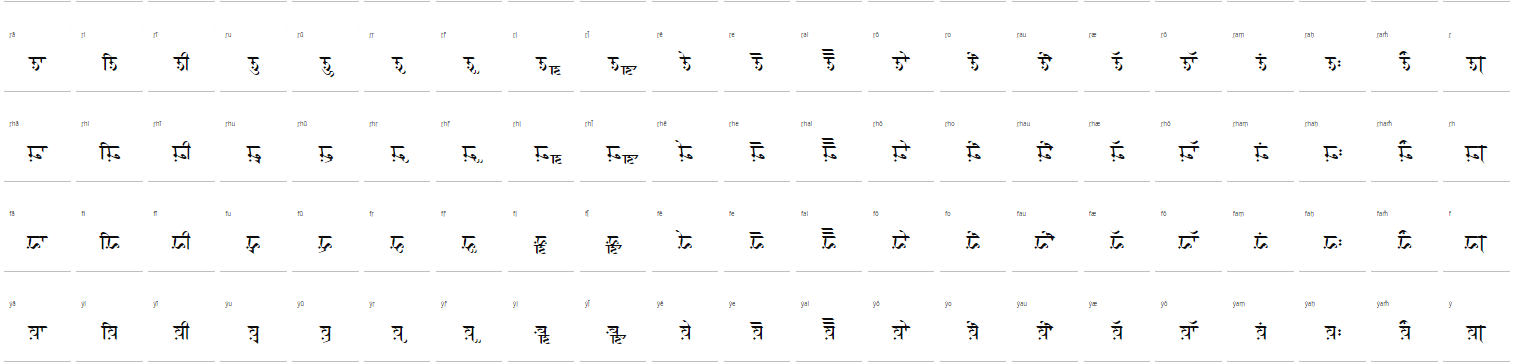
\includegraphics[width=\linewidth,keepaspectratio]{sharada_compounds_ra_varga} 
	
	{\tiny (Ref: Aksharamukha : Script Converter)}
	\end{center}	

\end{frame}

\section[Trans]{Transliteration}
%%%%%%%%%%%%%%%%%%%%%%%%%%%%%%%%%%%%%%%%%%%%%%%%%%%%%%%%%%%%%%%%%%%%%%%%%%%%%%%%%%
\begin{frame}[fragile]\frametitle{}
\begin{center}
{\Large Transliteration}
\end{center}
\end{frame}


%%%%%%%%%%%%%%%%%%%%%%%%%%%%%%%%%%%%%%%%%%%%%%%%%%%%%%%%%%%
\begin{frame}[fragile]\frametitle{Aksharamukha : Script Converter}


	\begin{lstlisting}
pip install aksharamukha

from aksharamukha import transliterate
transliterate.process(src, tgt, txt, nativize = True, pre_options = [], post_options = [])
transliterate.process('HK', 'Telugu', 'buddhaH')

# If the source script is not known, set it as autodetect
transliterate.process('autodetect', 'IAST', '....')

# You can also convert files (.docx, .html & .txt) as shown below.
from aksharamukha import transliterate_file
transliterate_file.process(src, tgt, file_path, nativize=True, pre_options = [], post_options = [])


# REST API
http://aksharamukha-plugin.appspot.com/
api/public?source=HK&target=Telugu&text=buddhaH
\end{lstlisting}

\end{frame}




\section[End]{Towards End}
%%%%%%%%%%%%%%%%%%%%%%%%%%%%%%%%%%%%%%%%%%%%%%%%%%%%%%%%%%%%%%%%%%%%%%%%%%%%%%%%%%
\begin{frame}[fragile]\frametitle{}
\begin{center}
{\Large References}
\end{center}
\end{frame}


%%%%%%%%%%%%%%%%%%%%%%%%%%%%%%%%%%%%%%%%%%%%%%%%%%%%%%%%%%%
\begin{frame}[fragile]\frametitle{References}

Many publicly available sources have been used in the preparation of this content. Some of the salient ones are listed below:

	\begin{itemize}
	\item Core Sharada Team https://www.shardalipi.com/ Courses, Resources
	\item Learn Sharada Lipi - Learn Sanskrit Online : vyoma-samskrta-pathasala YouTube % https://www.youtube.com/playlist?list=PLmozlYyYE-ETiEDyzg3UYg4pbNz31nCEG
	\item Virtual Vinodh http://www.virtualvinodh.com/projects Transliteration code Github
	\item Satisar https://satisarsharada.appspot.com/editor Online Transliteration App
	\item Sharada script translation - Kashmiri Youth Movement https://kashmiriyouthmovement.org/sharada-script-translation/
	\item Sarada script | South Indian, Tamil-Brahmi, Grantha | Britannica https://www.britannica.com/topic/Sarada-script
	\item Kashmiri transliteration - Wikipedia https://en.m.wikipedia.org/wiki/Kashmiri\_transliteration
	\item Noto Sans Sharada - Google Fonts https://fonts.google.com/noto/specimen/Noto+Sans+Sharada
	\item Shaarda - Sunil M YouTube %https://www.youtube.com/playlist?list=PLkTrUAJaxE7A\_OYBGu2hAXvuMkwZ\_JYWe
	\end{itemize}

\end{frame}


%%%%%%%%%%%%%%%%%%%%%%%%%%%%%%%%%%%%%%%%%%%%%%%%%%%%%%%%%%%
\begin{frame}[fragile]\frametitle{}

\begin{center}
\includegraphics[width=0.8\linewidth,keepaspectratio]{my_yog_back}

Thanks धन्यवाद
\end{center}

\end{frame}

	
	\begin{frame}[c]{}
	Thanks ...
	\vspace{5mm}
	yogeshkulkarni@yahoo.com
	\end{frame}

\end{document}
